\section{Sensorik und Sicherheitstechnik \textcolor{gray}{(Elena Widmann)}}
\label{sec:Sensorik und Sicherheitstechnik}

\subsection{Sensorik}
\label{sec:Sensorik}
\subsubsection{Aufgabenstellung}
Die Sensorik soll so ausgelegt sein, dass eine langjährige, korrekte und sichere Funktion des AFSS gewährleistet wird. Die einzelnen Sensoren sollen ihren Aufgaben entsprechend ausgewählt werden. Außerdem sollen, wenn möglich, bereits verfügbare Komponente verwendet werden, um Kosten zu minimieren. Falls dies nicht möglich ist, soll eine Lösung gefunden werden, die die gegebenen Anforderungen bestmöglich erfüllt. Zusätzlich muss ein passendes Feldbussystem gewählt werden, um eine reibungslose Kommunikation zwischen den Sensoren und der SPS sicherstellen zu können. Die Sensorik ist dafür zuständig, die Entstehung von Schäden am System nicht nur zu vermeiden, sondern gar nicht erst zuzulassen.

\subsubsection{Endschalter}
Beim Verplanen der Endschalter ist zwischen Software- und Hardware-Endschalter zu unterscheiden. Die Software-Endschalter begrenzen den Arbeitsbereich der Achse und sollten innerhalb des Bereichs der Hardware-Endschalter parametriert werden. Ihre Positionen werden direkt im Siemens TIA-Portal eingestellt und können falls notwendig einfach auf die aktuelle Geschwindigkeit angepasst werden. Werden die Software-Endschalter angefahren, wird der Technologiealarm 533 ausgelöst und die Dynamikwerte gestoppt, das Technologieobjekt bleibt hierbei freigegeben. Werden sie jedoch überfahren, wird das Technologieobjekt gesperrt. \\
Die Hardware-Endschalter begrenzen den maximal zulässigen Verfahrensbereich der Achse. Bei ihnen wird nicht unterschieden, ob die Endschalter angefahren oder überfahren werden. Beim Anfahren der Schalter wird der Technologiealarm 531 ausgelöst. Er sperrt das Technologieobjekt und muss, bevor der Auslösebereich der Hardware-Endschalter wieder verlassen werden kann, quittiert werden. \cite{axis_manual}\\
Auf jeder der drei Achsen des AFSS, und auf dem Querförderer, müssen Hardware-Endschalter montiert werden. Die Auswahl der Endschalter begrenzte sich auf die dem AFSS zur Verfügung gestellten Sensoren, welche unter Berücksichtigung ihrer Funktion auf den verschiedenen Positionen eingebaut wurden.

\paragraph{Positionsschalter mit Rollhebel} \mbox{}\\
An der x-Achse werden als Hardware-Endschalter Positionsschalter mit Rollhebel verwendet (siehe Abb. \ref{roll_sens}). Von den insgesamt vier Stück werden zwei an der unteren und zwei an der oberen x-Achse befestigt. Davon besitzen drei jeweils einen Öffner- und einen Schließerkontakt, wohingegen einer der Endschalter aus zwei Öffnerkontakten besteht. Um Einheitlich zu bleiben, und da es sicherheitstechnisch auch von Vorteil ist (Drahtbruchsicherheit), wird jeweils einer der Öffnerkontakte der Endschalter verwendet. Zum Schalten des Rollhebels der Positionsschalter müssen auf dem x-Schlitten der oberen sowie unteren x-Achse Auslöser angebracht werden. Diese befinden sich mittig auf der Seite der Sensoren und gleichen einem vom Schlitten abstehenden Arm, welcher sich aus gestapelten, mit dem Lasercutter gefertigten, Teilen zusammensetzt.

\paragraph{Induktive Endschalter} \mbox{}\\
Als Hardware-Endschalter an der y-Achse werden induktive Sensoren verwendet (siehe Abb. \ref{ind_sens}). Davon werden zwei an der unteren und zwei an der oberen Seite der y-Achse befestigt, somit handelt es sich auch hier wieder um vier Sensoren. Sie funktionieren so, dass durch eine Spule ein Magnetfeld erzeugt wird, welches dann in einem sich dem Sensor frontseitig nähernden elektrisch leitendem Material Wirbelströme erzeugt. Dadurch verändert sich das Magnetfeld und die Kontakte des induktive Sensors werden über einen Schmitt-Trigger geschaltet. Die Sensoren besitzen jeweils einen Öffner- und einen Schließerkontakt, es wird jedoch ersteres verwendet, um Drahtbruchsicherheit zu gewährleisten. Damit die induktiven Sensoren korrekt auslösen können, müssen auf dem Shuttle der y-Achse elektrisch leitende Gegenstücke angebracht werden.

\paragraph{Endtaster} \mbox{}\\
An der yz-Achse werden vier Stück, und am Querförderer zwei Stück, mechanische Endtaster als Endschalter verwendet. Auf einem Endtaster befindet sich ein Schließerkontakt in Form eines Tasters, welcher durch Anfahren geschaltet wird (siehe Abb. \ref{tast_sens}). Zum Betätigen der Taster müssen sich Auslöser auf dem Shuttle und den Seiten der Querfördererstation befinden.\\

\begin{figure}[H]
    \centering
    \begin{subfigure}{.3\textwidth}
        \centering
        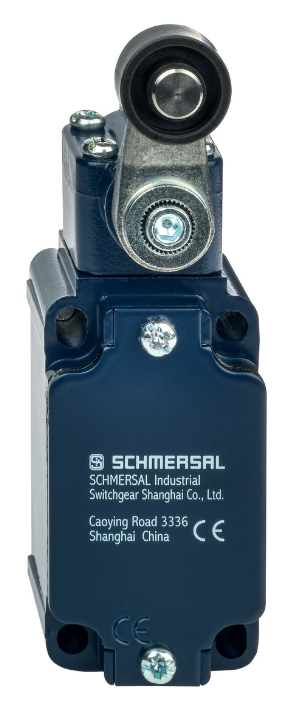
\includegraphics[width=0.5\textwidth]{Sensors/Rollendschalter.png}
        \caption{Rollendschalter,\\ Quelle: \cite{schmersal_pic}}
        \label{roll_sens}
    \end{subfigure}%>
    \begin{subfigure}{.3\textwidth}
        \centering
        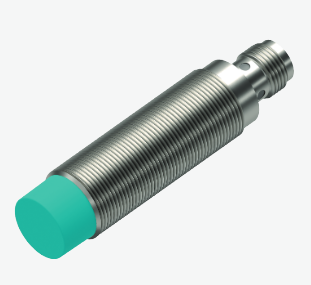
\includegraphics[width=1\textwidth]{Sensors/Induktiver_Sensor.png}
        \caption{Induktiver Sensor,\\ Quelle: \cite{induktiv_sensor}}
        \label{ind_sens}
    \end{subfigure}%
    \begin{subfigure}{.3\textwidth}
        \centering
        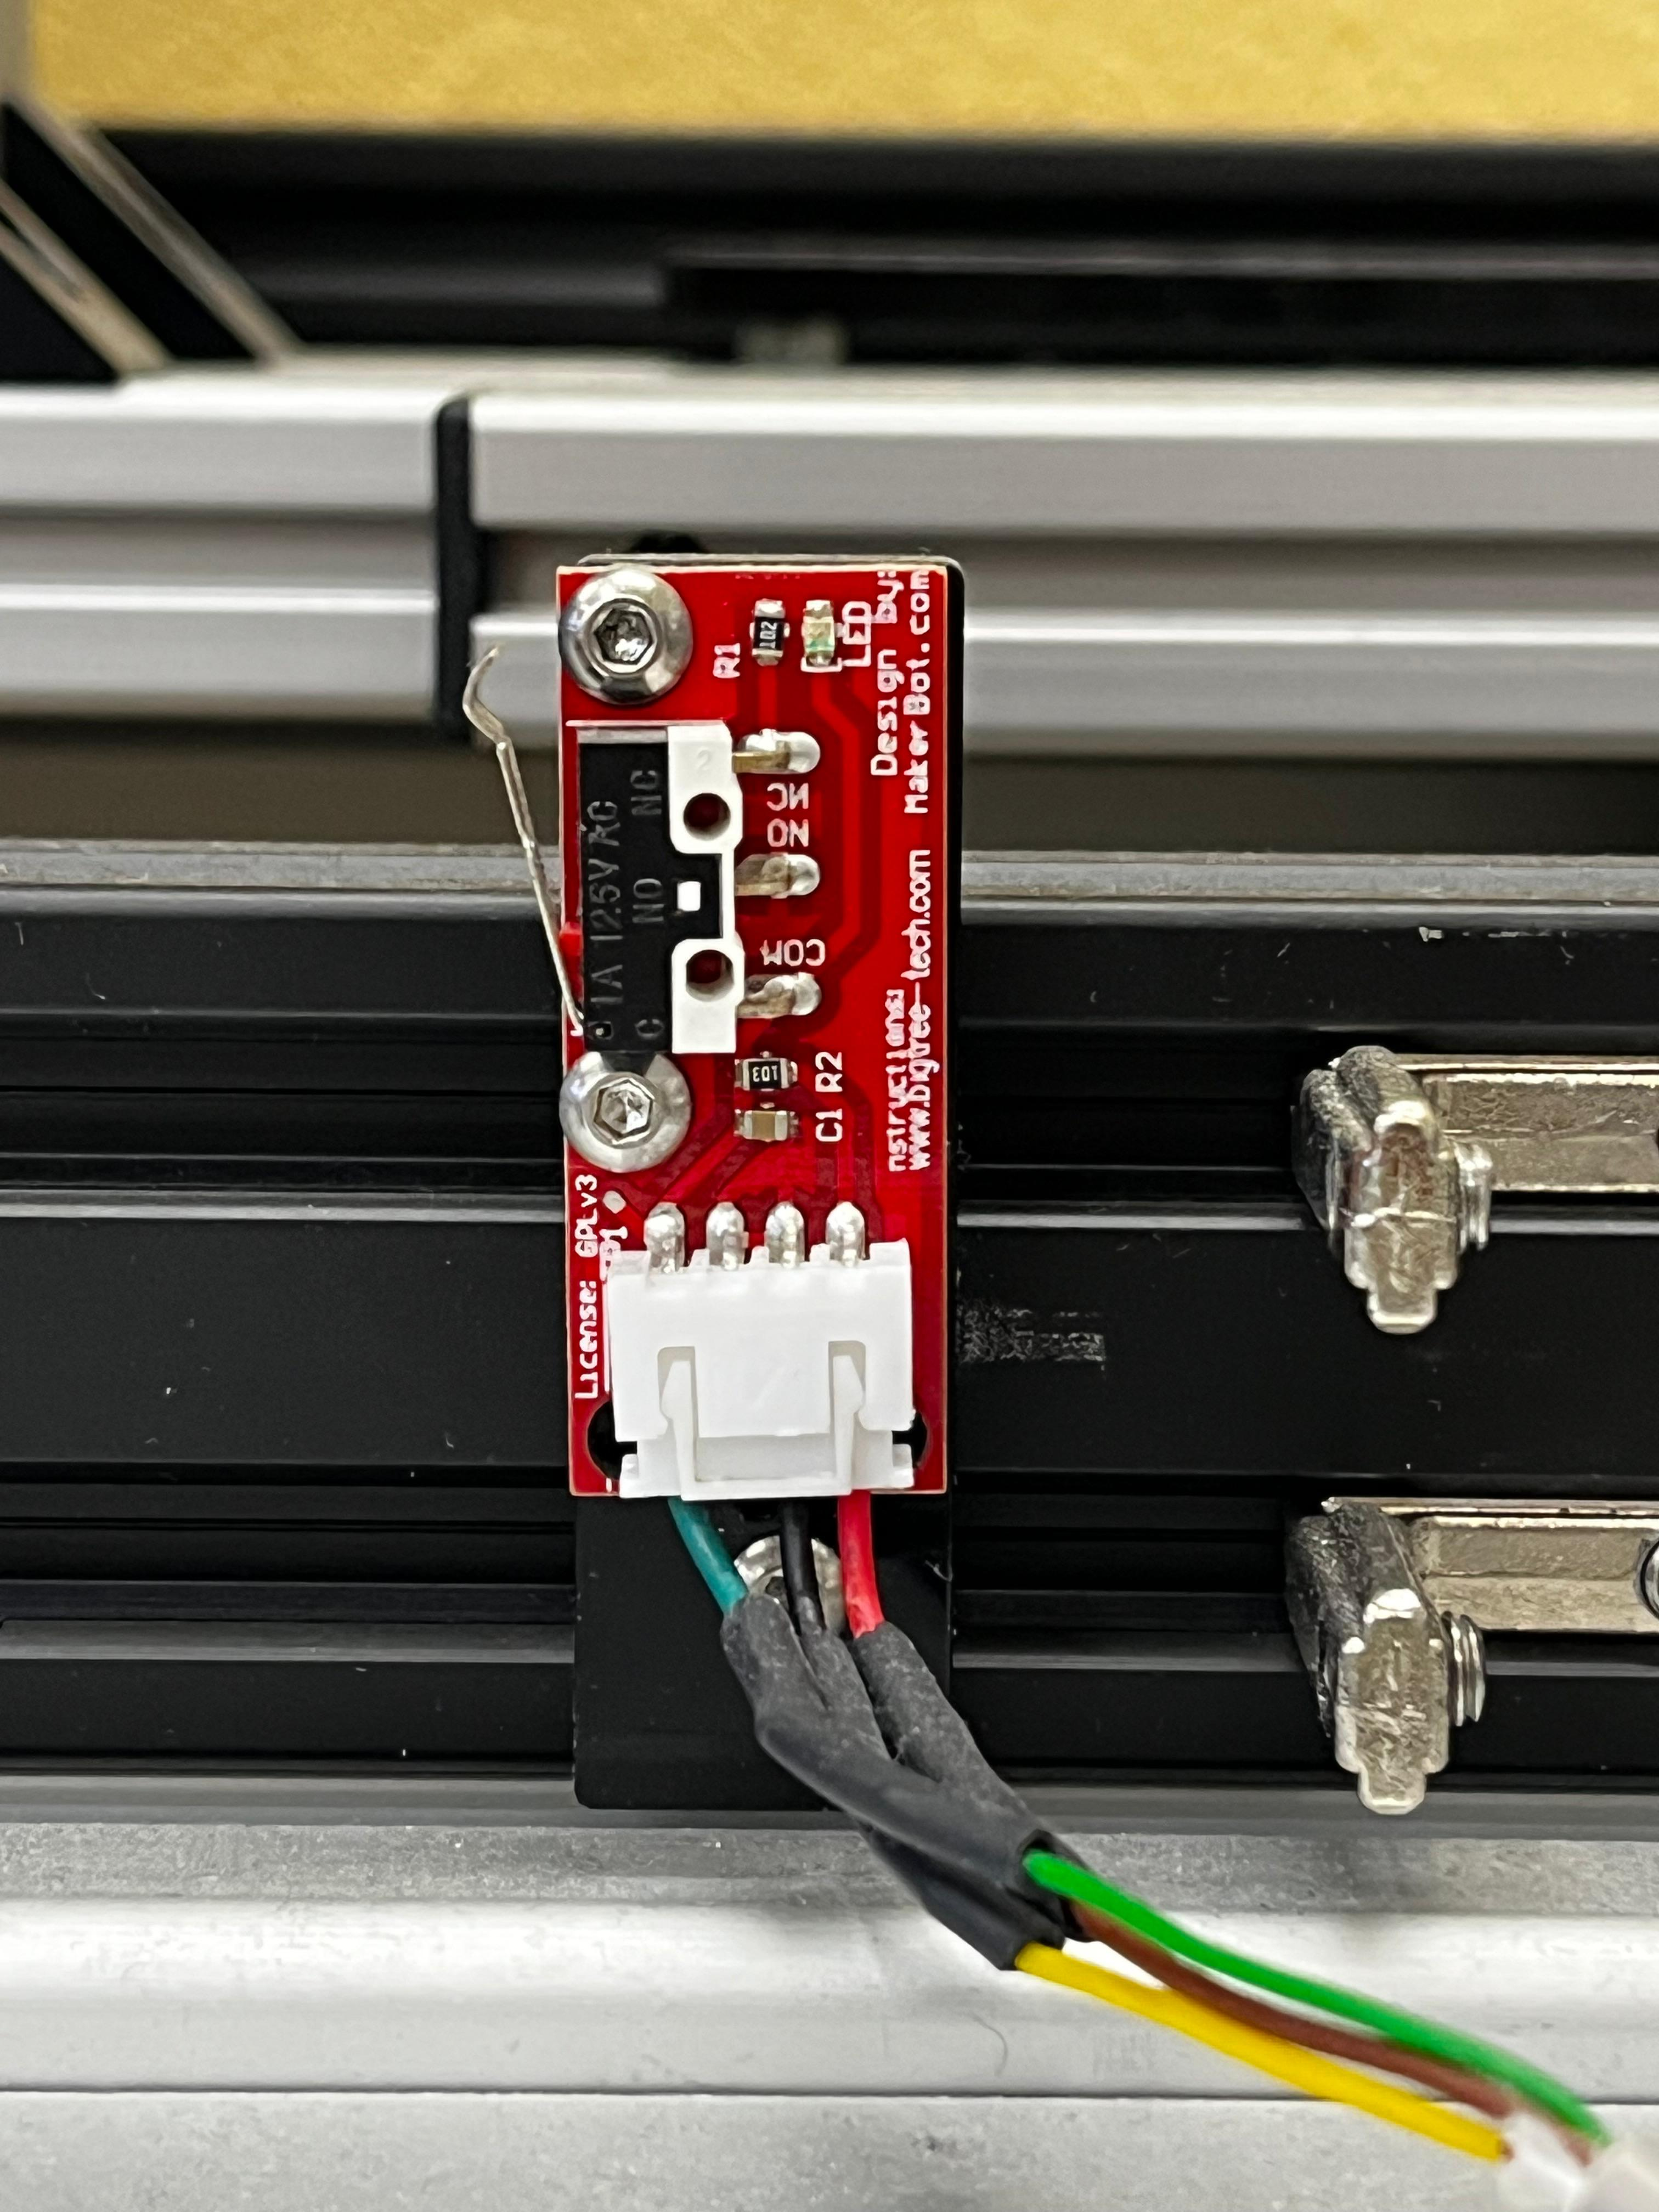
\includegraphics[width=0.9\textwidth]{Sensors/Endtaster.jpg}
        \caption{Endtaster}
        \label{tast_sens}
    \end{subfigure}
    \caption{Endschalter}
\end{figure}

\subsubsection{Referenztaster}
Um die Motoren auf die richtige Position fahren zu können, müssen diese an allen drei Achsen und am Querförderer referenziert werden. Durch stetiges Referenzieren wird dafür gesorgt, dass sich die Koordinaten der Positionen, auf denen sich die Bauteilboxen befinden, nicht verändern und es zu keiner Kollision zwischen Shuttle und einer Box bzw. dem Gerüst kommt. Nach einem Neustart des AFSS ist das erneute Referenzieren besonders wichtig.\\
Zum Referenzieren müssen Sensoren an den Achsen und am Querförderer angebracht werden, welchen den jeweiligen Nullpunkt angeben. Hierfür werden Opto Interrupter verwendet, da diese einfach durch anfahren ausgelöst werden können. In einem Opto Interrupter befindet sich eine LED, dessen Lichtstrahl auf einen Photo Transistor trifft. Dieser schaltet daraufhin durch und es liegt eine Spannung am Emitter an. Wird jetzt jedoch der Lichtstrahl der LED unterbrochen, sperrt der Transistor und es fließt kein Strom. Bei der SPS-Programmierung ist daher zu beachten, dass sich der Ausgang des Sensors im nicht geschalteten Zustand auf HIGH befindet. Wird der Lichtstrahl jedoch unterbrochen, liegt am Sensorausgang keine Spannung an und der Eingang der SPS erhält ein LOW Signal.\\
Damit während eines Referenziervorgangs der Lichtstrahl der LED unterbrochen wird und der Referenztaster auslöst, müssen auch hier wieder Auslösevorrichtungen an den beiden x-Schlitten, am Shuttle und an der Querfördererstation angebracht werden.\\
Für das AFSS werden TP808 zum Referenzieren verwendet. Hierbei ist zu beachten, dass die sich darin befindende Diode nur mit einer maximalen Flussspannung von \qty{1.35}{\volt} betrieben werden darf.\cite{TP808} Da die Opto Interrupter jedoch über ASi-Bus mit der SPS verbunden werden, welche eine Spannung von \qty{24}{\volt} liefert, musste eine eigene Platine entworfen und hergestellt werden, um das Bauteil nicht mit einer zu hohen Betriebsspannung zu zerstören. Hierfür wurde die Software Fusion360 verwendet, welche das Designen von Leiterplatten ermöglicht. Hergestellt wurden diese dann durch die schulinterne Leiterplattenfertigung der HTL Mössingerstraße. Insgesamt musste die Referenzplatine sieben mal hergestellt werden.

\paragraph{Schaltungsentwurf} \mbox{}\\
Die Schaltung musste so konzipiert werden, dass keines der involvierten Bauteile über längeren Normalbetrieb oder durch kurzzeitige hohe Ströme bzw. Spannungen, beschädigt wird. Das Ziel ist, die korrekte Funktion des Opto Interrupters auch zukünftig noch sicher stellen zu können. Dafür ist besonders wichtig auf dessen elektrische Eigenschaften zu achten, welche im Datenblatt zu finden sind. Für den fertigen Entwurf der Schaltung siehe Abb. \ref{Ref_Schaltplan}.\\
Im Opto Interrupter befindet sich eine LED mit einer maximalen Durchlassspannung von \qty{1.35}{\volt}. und einer typischen Durchlassspannung V$_{F}$ von \qty{1.2}{\volt}. Um diese nicht mit den vollen \qty{24}{\volt} der Betriebsspannung V$_{B}$ zu überlasten muss ein Vorwiderstand R$_{1}$ eingebaut werden. Um die LED zum leuchten zu bringen, soll ein minimaler I$_{F}$ von \qty{10}{\milli\ampere} fließen. Dann lässt sich daraus der Vorwiderstand aus dem ohmschen Gesetz und mit Hilfe der Maschenregel berechnen:

\begin{equation*}
    R_{1} = \frac{V_{B} - V_{F}}{I_{F}} = \frac{\qty{24}{\volt} - \qty{1.2}{\volt}}{\qty{10}{\milli\ampere}} = \qty{2.28}{\kilo\ohm}
\end{equation*}

In der HTL wird den Schülerinnen und Schülern die Widerstandsreihe E12 zur Verfügung gestellt. Daher wird in der Schaltung der nächstgrößere Widerstand mit dem Wert $\qty{2,7}{\kilo\ohm}$ verwendet.\\
Der Phototransistor, welcher als Gegenstück zur LED dient, darf mit einer maximalen Collector-Emitter-Spannung von \qty{30}{\volt} betrieben werden, wodurch er gut geeignet ist für das Ziel der Schaltung. Um jedoch im besten Fall die gesamten \qty{24}{\volt} für den Eingang der SPS an der Klemme X1 abgreifen zu können, wird ein Spannungsteiler verwendet, bei dem nach dem Transistor ein Widerstand R$_{3}$ parallel zur Klemme X1 eingebaut wird. Da nur ein niedriger Strom benötigt wird, kann I$_{R3}$ relativ klein sein, hier \qty{1}{\milli\ampere}. Daraus lässt sich dann der Widerstandswert wie folgt berechnen:

\begin{equation*}
    R_{3} = \frac{V_{B}}{I_{R3}} = \frac{\qty{24}{\volt}}{\qty{1}{\milli\ampere}} = \qty{24}{\kilo\ohm}
\end{equation*}

Auch hier wird wieder der nächstgrößere Widerstandswert, der zur Verfügung gestellt wird, verwendet. R$_{3}$ entspricht somit dem Wert $\qty{27}{\kilo\ohm}$.\\
Für Funktionstests und die Inbetriebnahme ist es wichtig, dass eine Möglichkeit gegeben ist, den Zustand des Ausgangs der Schaltung anzuzeigen. Hierfür wird eine grüne 5mm LED verwendet, welche parallel zur Klemme X1 eingebaut wird. Da der Transistor einen maximalen Collector Strom von \qty{20}{\milli\ampere} besitzt, wurde die Entscheidung getroffen, die grüne LED nur mit \qty{10}{\milli\ampere} zu versorgen, da diese auch bei geringerem Strom genug Leuchtkraft für den benötigten Zweck besitzt. Bei einem Strom I$_{R2}$ von \qty{10}{\milli\ampere} besitzt die LED einen Spannungsabfall V$_{LED}$ von \qty{2.1}{\volt}.\cite{led_grün} Daraus lässt sich dann er Widerstand R$_{2}$ berechnen:

\begin{equation*}
    R_{2} = \frac{V_{B} - V_{LED}}{I_{R2}} = \frac{\qty{24}{\volt} - \qty{2.1}{\volt}}{\qty{10}{\milli\ampere}} = \qty{2.19}{\kilo\ohm}
\end{equation*}

Der nächsthöhere Widerstand der E12 Reihe entspricht $\qty{2,2}{\kilo\ohm}$, um auf Nummer sicher zu gehen wird jedoch der um eine Stufe größere Widerstand mit einem Wert von $\qty{2,7}{\kilo\ohm}$ verwendet. Wenn der Lichtstrahl im Opto Interrupter nicht unterbrochen wird und der Transistor somit durchschaltet, leuchtet die grüne LED. Wird jetzt der Lichtstrahl unterbrochen erlischt die LED. Damit diese nicht während des Normalbetriebs dauerhaft leuchtet wird ein Jumper eingebaut, durch dessen Entfernung die LED ganz einfach aus der Schaltung ausgeschlossen werden kann.

\begin{figure}[H]
    \centering
    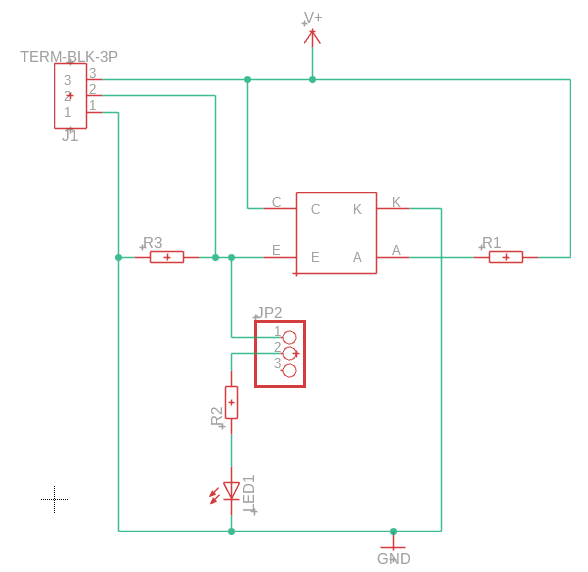
\includegraphics[width=0.8\textwidth]{Sensors/Ref_Schaltplan.png}
    \caption{Schaltplan Referenzplatine}
    \label{Ref_Schaltplan}
\end{figure}

\paragraph{Platinenentwurf und -herstellung} \mbox{}\\
Um die benötigten Referenzplatinen herstellen zu können, musste zuerst ein Leiterplattenplan in Fusion360, ehemals Eagle, erstellt werden. Über den Sharepoint der HTL lässt sich eine Elektronikbibliothek, die alle in der Schule verfügbaren Bauteile beinhaltet, herunterladen. Da der in der Schaltung verwendete Opto Interrupter nicht in der Schule verfügbar ist, sondern extern organisiert werden musst, befindet er sich nicht in dieser Elektronikbibliothek. Daher musste für ihn ein eigenes Symbol sowie ein dazugehöriger Footprint gezeichnet werden.\\
Zum Entwerfen eines Printed Circuit Boards (PCB) muss ein neuer Elektronikentwurf in Fusion erstellt werden. Hier muss zu Beginn der zugehörige Schaltplan gezeichnet werden. Wichtig ist, dass bei der dreipoligen Schraubklemme (J1) das Bauteil 3282837-3 verwendet wird, da sonst die Abstände zwischen den Lötpads zu klein und diese zu nah bei einander sind. Damit der Jumper (JP2) nicht verloren geht, wenn die Verbindung zwischen Ground und LED durch dessen Entfernung aufgehoben werden soll, wird ein dreipoliger Pinheader verwendet, um den Jumper für den gegebenen Zeitraum einfach umstecken zu können.\\
Nach Fertigstellung des Schaltplans kann in Fusion ein passendes Leiterplattendokument erstellt werden, welches die Bauteile und die zugehörigen Verbindungen direkt übernimmt. Für den fertigen Leiterplattenplan des Referenztasters siehe Abb. \ref{Ref_LPPlan}. Da beim verwendeten Opto Interrupter Löcher zur Montierung vorhanden sind, mussten auf der Platine selbst keine zusätzlichen Bohrungen eingeplant werden. Bei der Anordnung der Bauteile auf der Platine war zu beachten, dass sich die Löcher am Opto Interrupter am schmäleren rand der Platine befinden. Um eine leichtere Verkabelung zu ermöglichen, wurde auch die Schraubklemme am Rand der Platine platziert.

\begin{figure}[H]
    \centering
    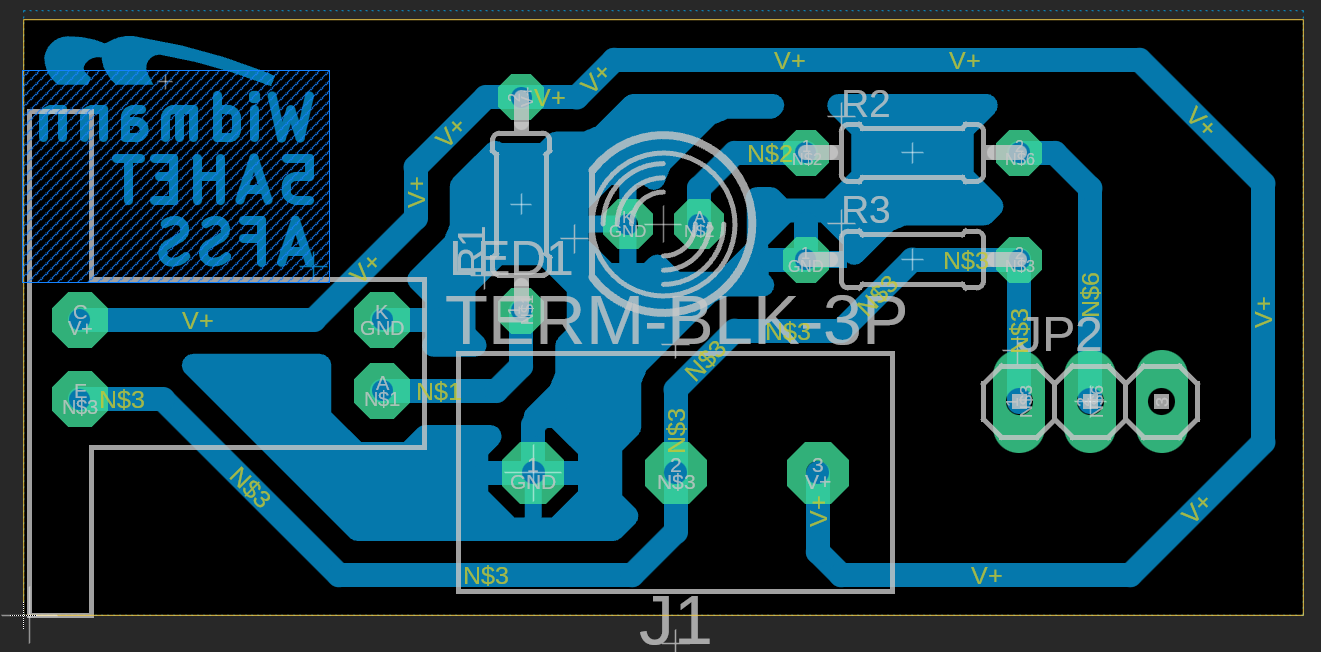
\includegraphics[width=0.7\textwidth]{Sensors/Ref_Leiterplattenplan.png}
    \caption{Leiterplattenplan Referenzplatine}
    \label{Ref_LPPlan}
\end{figure}

Wenn die Bauteile alle platziert und verbunden worden sind, sowie ein Polygon über die gesamte Platine gezogen worden ist, muss diese noch auf Fehler geprüft werden. Auch hier ist eine bereits fertige Datei, welche die benötigten Design Rules für Fusion360 beinhaltet, auf der Schulwebsite zu finden. Wichtig ist, damit die Platine zur Produktion in der Leiterplattenfertigung der HTL eingereicht werden kann, muss diese den vorgegebenen Anforderungen entsprechen. Dazu gehört, dass sich das HTL-Logo auf der Platine befindet und die Texteinstellungen Font: Vector, Ratio: \qty{16}{\percent} und Size: min \qty{70}{mil} entsprechen. Auch die Breite der Kupferbahnen darf nicht zu klein sein (hier: \qty{32}{mil}).\\
Nach Einreichung eines Fertigungsauftrags wird die Platine von Schülerinnen und Schülern der HTL gefertigt. Der Herstellungsprozess startet mit dem Reinigen des Basismaterials, um es daraufhin mit dem Negativtrockenresist (Trockenfilm) zu laminieren. In den nächsten Schritten werden die Layout-Informationen mit einem Belichter auf das Laminat übertragen und das unbelichtete Laminat mit einer Natrium-Carbonat Lösung von der Platine entfernt. Daraufhin werden, durch Ätzen mit einer Eisen-III-Chlorid-Lösung, strukturierte Kupferflächen freigestellt. Als Nächstes werden die Löcher in die Kupferpads gebohrt und die Platine auf ihre korrekte Größe zugeschnitten. Durch das Legen der Leiterplatte in eine Entschichtlösung aus \qty{5}{\percent}{igem} Kaliumcarbonat mit Wasser, werden Ätzresiste von der Platine entfernt. Zu guter Letzt wird die Platine mit einem Versiegelungslack versiegelt, um sie vor Umwelteinflüssen und Korrosion zu schützen.

\paragraph{Platinentestung und Messung} \mbox{}\\
Um die korrekte Funktionsweise der Referenzplatine sicherstellen zu können, musste diese nach dem Löten getestet werden. Zum Betrachten der fertigen Platine siehe Abb. \ref{Ref_fertig}. An der Klemme X1 wurden mit einem Multimeter Spannungswerte zwischen \qtyrange{19.7}{21.3}{\volt} gemessen. Obwohl die Spannungen unter den gewünschten \qty{24}{\volt} liegen, können die Platinen problemlos verwendet werden, da die verwendeten AS-i-Slaves einen minimalen HIGH-Eingangsschaltpegel von \qty{10}{\volt} besitzen.\cite{AS-i-Slave}

\begin{figure}[H]
    \centering
    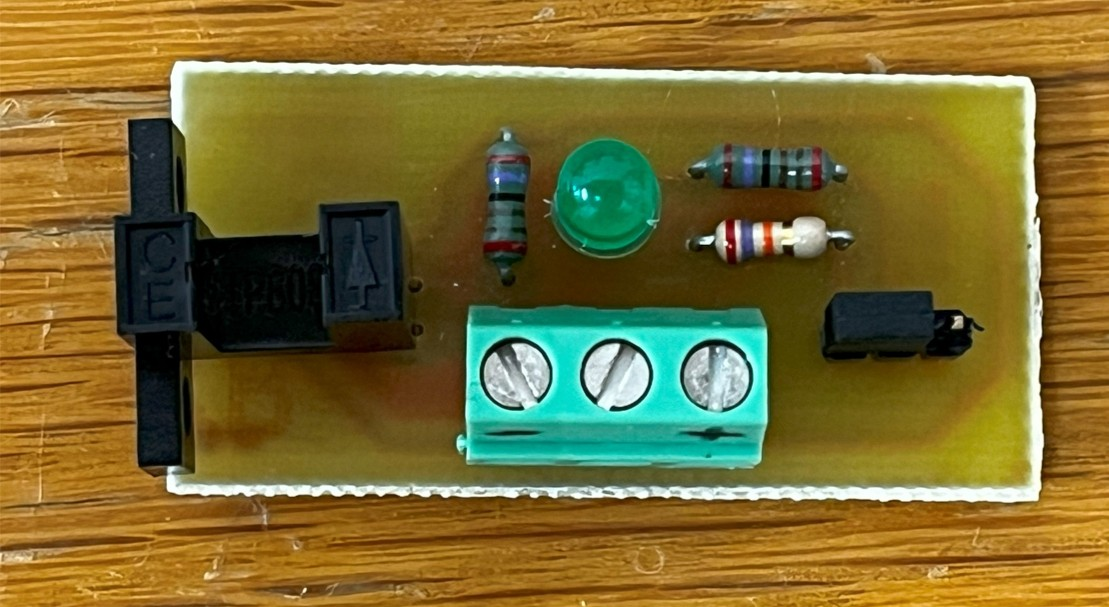
\includegraphics[width=0.5\textwidth]{Sensors/ref_FertigePlatine.jpg}
    \caption{Fertige Referenzplatine}
    \label{Ref_fertig}
\end{figure}

\subsubsection{Lichttaster}
Zum Überprüfen, ob während des Ein- oder Auslagerns eine Box auf der richtigen Position angekommen ist, werden Lichttaster verwendet. Insgesamt werden zwei am AFSS montiert, davon einer an der z-Achse und einer am Querförderer. Es handelt sich bei den hierbei verwendeten Reflexionslichttastern um Sensoren der Firma SICK vom Typ W4 WTBxx (siehe Abb. \ref{lichttaster}).\\
Ursprünglich hätte diese Aufgabe von Lichtschranken übernommen werden sollen, da diese bereits vor Ort verfügbar waren. Lichtschranken funktionieren, indem sie einen Rotlichtstrahl auf einen Reflektor werfen, dessen Reflektion daraufhin wieder vom Sensor erkannt wird. Im Lichtschranken befinden sich Schaltkontakten, die daraufhin geöffnet oder geschlossen werden. Wird nun jedoch der Lichtstrahl unterbrochen, fallen die Schaltkontakte in ihren Anfangszustand zurück. Die Lichtschranken haben jedoch den Nachteil, dass sie immer ein zusätzliches reflektierendes Gegenstück benötigen. Die stattdessen verwendeten Lichttaster mit Hintergrundausblendung funktionieren nach dem selben Prinzip, jedoch bieten sie den Vorteil, dass sie auch die Distanz des Objektes zum Sensor erfassen. Somit können Objekte unabhängig von ihrer Farbe und Oberfläche erkannt werden, soweit sie sich innerhalb des einstellbaren Tastbereiches befinden.\cite{Lichttaster_und_Schranken} Der empfohlene Schaltabstand des Lichttasters liegt zwischen \qtyrange{40}{140}{\milli\meter}, wodurch er sich für die Aufgaben im Projekt ideal eignet. Über die Teach-in Funktion des Sensors lässt dieser sich ganz einfach durch drücken der Teach-Taste auf den richtigen Schaltabstand einstellen.\cite{Lichttaster_datasheet}\\
Während das SPS-Programm von der CPU durchlaufen wird, überprüft dieses immer an den jeweiligen Zwischenschritten, ob es ein Signal des zuständigen Lichttasters erhalten hat, bevor das Programm fortgesetzt wird. Somit wird sichergestellt, dass die Boxen im Querförderer richtig positioniert worden sind und von der z-Achse richtig gegriffen werden können. Ansonsten könnte passieren, dass eine von der Gabel angehobene Box hinunterfällt, da diese nicht richtig positioniert war.

\begin{figure}[H]
    \centering
    \begin{subfigure}{.4\textwidth}
        \centering
        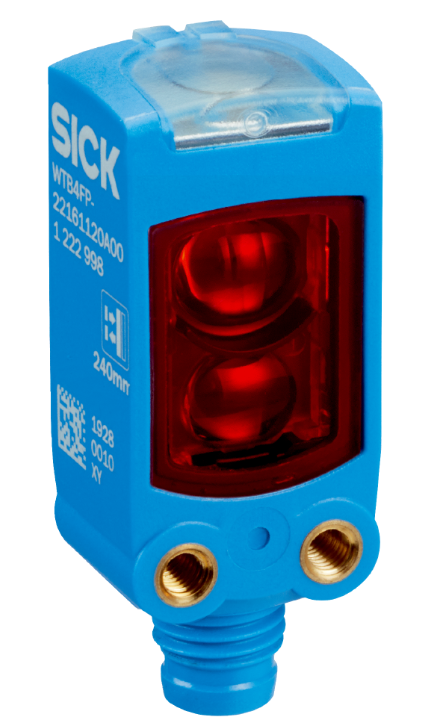
\includegraphics[width=0.4\textwidth]{Sensors/Lichttaster_new.png}
        \caption{Lichttaster W4 WTBxx,\\ Quelle: \cite{Lichttaster_pic}}
        \label{lichttaster}
    \end{subfigure}
    \begin{subfigure}{.4\textwidth}
        \centering
        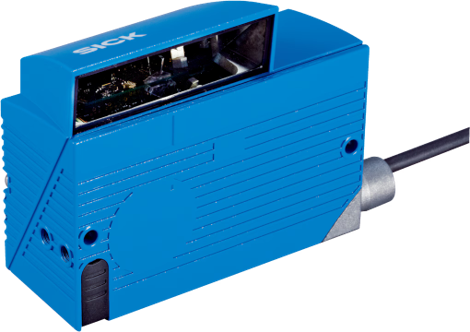
\includegraphics[width=0.8\textwidth]{Sensors/Barcodescanner.png}
        \caption{Barcodescanner CLV61x-2Port,\\ Quelle: \cite{BarScan_pic}}
        \label{BarScan}
    \end{subfigure}
    \caption{SICK Sensoren}
\end{figure}

\subsubsection{Barcode-Scanner} \label{sec:Barcodescanner}
Durch anbringen eines sich nicht wiederholenden Barcodes auf jeder Box wird eine gute Möglichkeit geschaffen, in der Software den Behälter und die sich darin befindenden Bauteile einander zuzuordnen. Unter der Voraussetzung, dass die Benutzerinnen und Benutzer vor jeder Wiedereinlagerung ihrer Box zuerst dessen Barcode einscannen, wird die Wahrscheinlichkeit, dass der Lagerplatz einer Box falsch abgespeichert wird, verringert. Somit sinkt auch die Chance, dass bei einer Bestellung ein falsches Bauteil ausgeliefert wird. Das erfassen des Barcodes findet mittels eines Barcodescanners der Firma SICK statt (siehe Abb. \ref{BarScan}). Dieser ist bei der Kommissionierstation untergebracht, um eine einfache Bedienung gewährleisten zu können.\\
Der dem AFSS zur Verfügung gestellte Barcodescanner (CLV61x-2Port) ist in der Lage alle gängigen Codearten einzulesen.\cite{Barcodescanner} Barcodes wurden so entwickelt, dass bereits beim Einlesen erkannt wird, wo dieser anfängt und aufhört, damit beim einscannen nicht auf die richtige Ausrichtung geachtet werden muss.

\paragraph{Einbindung ins TIA-Portal \cite{BarScan_Handbuch}}\mbox{}\\
Damit der eingelesene Barcode an den Webserver weitergegeben werden kann, muss dieser im Siemens TIA-Portal abgespeichert werden. Mit der CPU verbunden wird der Scanner über PROFINET. Hierbei handelt es sich um einen auf Industrial Ethernet basierenden Kommunikationsstandard und eine Weiterentwicklung des PROFIBUS Vorgängers. Für eine ausführlichere Erklärung der verschiedenen Feldbussysteme siehe Kapitel \ref{sec:Feldbussysteme}. Über ihn lässt sich die gescannte Nummer ganz einfach an die SPS übermitteln.\\
Im TIA-Portal Projekt muss, um eine Verbindung zum Barcodescanner herstellen zu können, die zugehörige Gerätebeschreibungsdatei (GSD-Datei) installiert werden. Dies funktioniert über das \enquote{Gerätebeschreibungsdateien verwalten} Fenster im TIA-Portal. Nach der Installation ist das Gerät im Hardwarekatalog unter \enquote{Weitere Feldgeräte} zu finden. Die benötigte Datei wird auf der Internetseite des Herstellers als Download zur Verfügung gestellt.

\paragraph{Auslesen des Barcodes}\mbox{}\\
Wenn eine Verbindung zum Gerät hergestellt wurde, müssen die Parametermodule eingefügt und richtig eingestellt werden. Diese werden über den Hardware-Katalog ausgewählt und in das Projekt gezogen, für eine Übersicht der eingefügten Module siehe Abb. \ref{BarScan_TIA}. Wichtig ist, bei den Baugruppenparametereinstellungen von \enquote{\mbox{47\_Communication Mode\_1}} \enquote{No Handshake} auszuwählen und bei \enquote{\mbox{99\_End Remote Config}}
\enquote{Don't save parameters perm.} einzustellen. Um die verwendeten Art von Barcodes einscannen zu können muss darauf geachtet werden, dass dieser unter \enquote{\mbox{22\_UPC EAN GTIN\_1}} ausgewählt und somit eingeschaltet sind.\\

\begin{figure}[H]
    \centering
    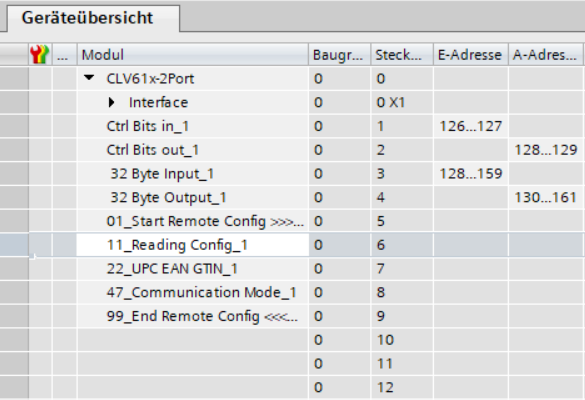
\includegraphics[width=0.6\textwidth]{Sensors/BarScan_Geräteübersicht.png}
    \caption{Barcodescanner Geräteübersicht im TIA-Portal}
    \label{BarScan_TIA}
\end{figure}

Die vom Barcodescanner belegten Ein- und Ausgangsadressen sind in der Geräteübersicht ersichtlich (siehe Abb. \ref{BarScan_TIA}). Ein TriggerBit wird verwendet um das Einlesen eines Barcodes zu starten, dabei handelt es sich um das zweite Bit des \enquote{\mbox{Ctrl Bits out\_1}} Moduls (hier: Q129.0). Bei steigender Flanke des ToggleBits wird der Laser eingeschaltet, erst bei der fallenden Flanke wird daraufhin der Code eingelesen.\\
Die eingelesenen Daten liegen ab dem ersten Input Byte (hier: ab IB128.0). Auf dem ersten Input Byte wird am vierten Bit ein ToggleBit mitgeführt. Am zweiten Byte(IB129.0) befindet sich ein Zähler, der mitzählt, wie viele Codes bereits eingelesen wurden. Das vierte Input Byte (IB131.0) gibt die Länge des eingelesenen Strings an. Ab dem sechsten Byte (IB133.0) stehen die eigentlichen Daten des Barcodes.\\
Um die Daten des Barcodes überprüfen zu können eignet sich eine wie in Abb. \ref{BarScan_BTabelle} abgebildete Beobachtungstabelle. Wichtig ist, dass beim Einfügen der Ein- und Ausgangsadressen das richtige Anzeigeformat ausgewählt ist. Um eine Überprüfung durchzuführen, lässt sich das TriggerBit zum Starten es Einlesevorgangs über Eingabe von TRUE und FALSE setzen, und daraufhin ein Code scannen. Die einzelnen Input Bytes werden daraufhin in der Tabelle angezeigt.

\begin{figure}[H]
    \centering
    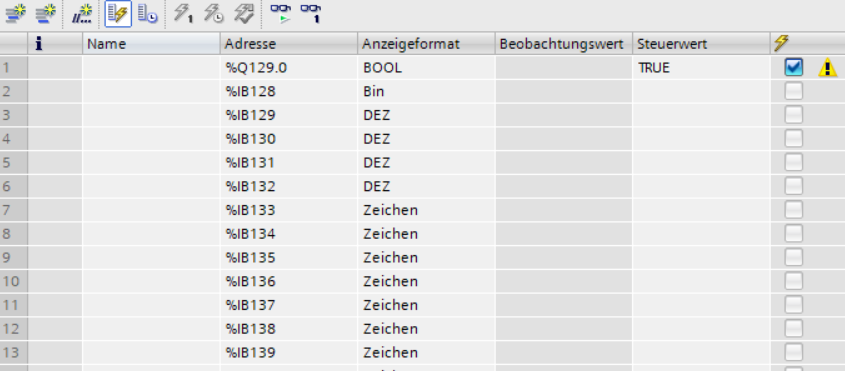
\includegraphics[width=0.9\textwidth]{Sensors/BarScan_Beobachtungstabelle.png}
    \caption{Barcodescanner Beobachtungstabelle im TIA-Portal}
    \label{BarScan_BTabelle}
\end{figure}

\subsection{AS-Interface}
\subsubsection[Feldbussysteme]{Feldbussysteme \cite{Feldbussysteme}} \label{sec:Feldbussysteme}
\paragraph{Allgemeines}\mbox{}\\
Ein Feldbus ist ein Bussystem, das Feldgeräte (Sensoren) und Stellglieder (Aktoren) mit einem Automatisierungsgerät, beispielsweise einer SPS, verbindet. Über den Feldbus findet die Kommunikation statt. Wenn die Nachrichten mehrerer Kommunikationsteilnehmer über die selbe Leitung gesendet werden, muss festgelegt sein, wer (Kennung), was (Messwert oder Befehl), wann (Initative) über den Bus sendet. Es existiert bereit eine Vielzahl an unterschiedlichen Bussystemen, zu den in der Automatisierungstechnik gebräuchlichsten gehören PROFIBUS, PROFINET, Industrial Ethernet, Modbus, AS-Interface, CANopen und EtherCAT. Da die verschiedenen Bussysteme unterschiedliche Datentransferzeiten und Fehlererkennungsmöglichkeiten bieten, werden oft in einem Projekt mehrere Feldbusse auf den verschiedenen Automatisierungsebenen verwendet. In Abb. \ref{Feldbussysteme} ist ein Beispielprojekt mit unterschiedlichen Bussystemen ersichtlich.\\

\begin{figure}[H]
    \centering
    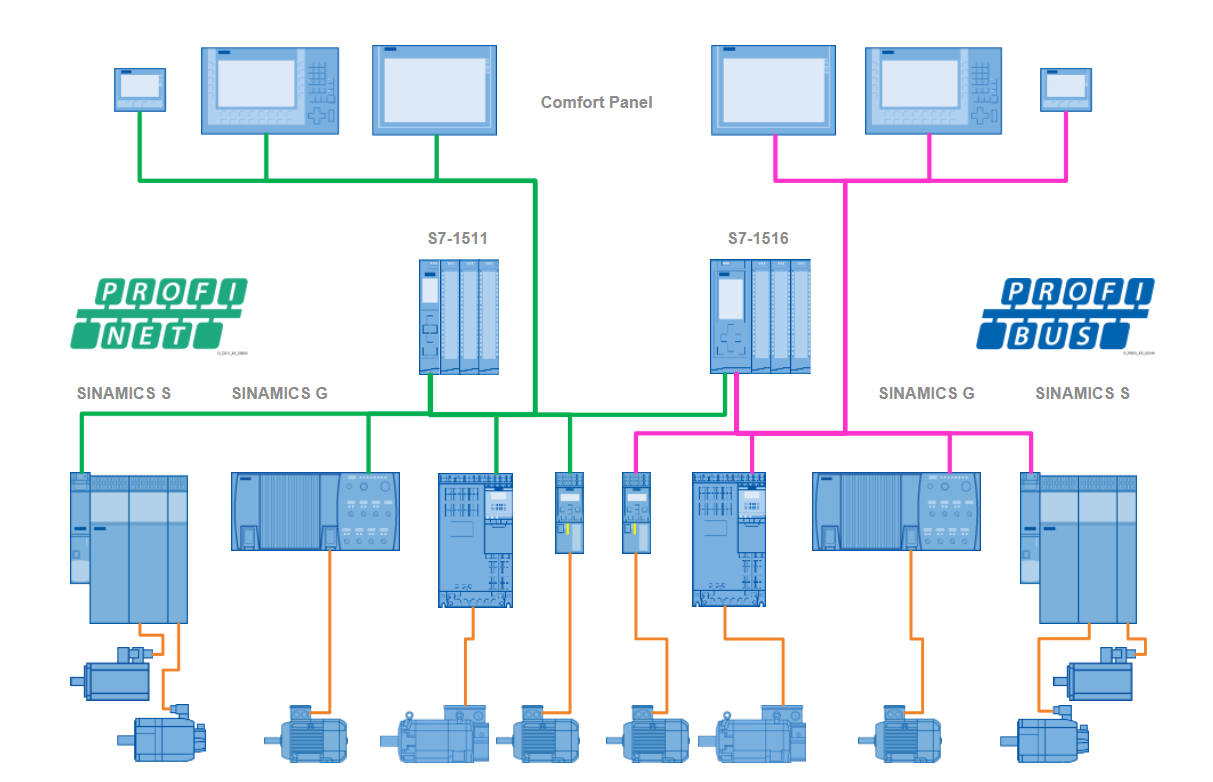
\includegraphics[width=0.7\textwidth]{Sensors/Feldbussysteme.png}
    \caption{Topologie verschiedener Feldbussysteme, Quelle: \cite{Topologie_Bussysteme}}
    \label{Feldbussysteme}
\end{figure}

\paragraph{PROFIBUS \cite{Profibus}}\mbox{}\\
Bei PROFIBUS (Process Field Bus) handelt es sich um ein standardisiertes Bussystem, das vor allem in der Automatisierungstechnik zu Hause ist. Es ist ein Multi-Master-System, das bedeutet, dass die Kommunikationsabläufe von mehreren Mastern gesteuert werden können. Die am häufigsten verwendete Schnittstelle in einem PROFIBUS-System ist RS485. Zur Datenübertragung wird meist ein 9-poliger Sub-D-Stecker verwendet. Die Anzahl der Teilnehmer ist je PROFIBUS SUB-Netz auf 32 beschränkt, somit ergibt sich eine maximale Anzahl von 128 Teilnehmern. PROFIBUS bietet den Vorteil, dass es sehr einfach in gängige Automatisierungssysteme integriert werden kann. Die Kabelfarbe ist violett, was auch beim Herstellen von PROFIBUS-Verbindungen im TIA-Portal ersichtlich ist.

\paragraph{PROFINET \cite{Profinet}}\mbox{}\\
Wie bereits in Kapitel \ref{sec:Barcodescanner} erwähnt wurde, handelt es sich bei PROFINET (Process Field Network) um eine Weiterentwicklung von PROFIBUS. Es basiert auf Industrial Ethernet und wurde von Siemens und den Mitgliedsfirmen der PROFIBUS-Nutzerorganisation entwickelt. PROFINET-Geräte werden ausschließlich über Switches miteinander verbunden, wobei viele Geräte, sowie eine SPS, bereits einen Switch mit mehreren Anschlüssen integriert haben. Der Vorteil von PROFINET ist, dass es das bekannte 7-schichtige OSI-Modell auf ein 4-schichtiges TCP/IP-Modell reduziert. Der Unterschied zum älteren PROFIBUS liegt vor allem darin, dass es die Funktion große Datenmengen übertragen zu können, bietet. Ein weiterer Vorteil ist die Echtzeitfähigkeit von PROFINET. Außerdem ist die Anzahl der Teilnehmer in einem PROFINET-System praktisch unbegrenzt, da jeder Teilnehmer eine eigene IP-Adresse besitzt. Bei der Projektierung im TIA-Portal müssen die Kommunikationspartner einem gemeinsamen PROFINET zugewiesen werden. Zusätzlich muss jedes Gerät einen PROFINET-Namen besitzen, die IP-Adresse des Geräts alleine genügt nicht. Die Kabelfarbe ist grün, was sich auch im TIA-Portal wiederspiegelt.

\paragraph{ASi \cite{ASi}}\label{par:ASi}\mbox{}\\
Bei ASi (Actuator-Sensor-Interface) handelt es sich um ein Feldbussystem, welches in der Automatisierungstechnik zur Verbindung von Sensoren und Aktoren mit einem Steuerungselement dient. Eingesetzt wird das AS-Interface in der Feldebene und findet vorwiegend bei Übertragung von Prozessdaten Verwendung. Es funktioniert nach dem Master-Slave-Prinzip, bei dem ein ASi-Master für die Kommunikation mit seinen Slaves zuständig ist. Der Datenverkehr findet hierbei in Form einer zyklischen Abfrage statt. In einem Zyklus sendet der Master Informationen an die Slaves, die daraufhin wieder eine Antwort zurücksenden. Der große Vorteil an ASi ist, dass die Daten- und Stromübertragung meist über ein einziges Kabel passiert. Hierbei handelt es sich um ein gelbes 2-adriges Profilkabel, in dem sich ein brauner (Plus) und ein blauer (Minus) Leiter befindet. Die Betriebsspannung eines ASi-Systems liegt bei \qty{30}{\volt}. Wenn ein Feldgerät eine zusätzliche Hilfsspannung (\qty{24}{\volt}) benötigt, wird ein schwarzes Profilkabel verwendet. Bei der Verwendung von ASi können durch die Reduzierung der benötigten Kabel die Installationskosten erheblich gesenkt werden. Außerdem ist die Verkabelung übersichtlicher und Verdrahtungsfehler können besser vermieden werden. Beim Anschließen eines Asi-Kabels an einem Feldgerät wird die Durchdringungstechnik verwendet. Dabei durchdringen bei der Montage zwei sich am Anschluss befindende Dornen die Isolierung des Kabels, und stellen darüber eine Verbindung zum Netzwerk her.

\paragraph{Auswahl des Feldbussystems}\mbox{}\\
Da es sich bei PROFINET um ein von Siemens mitentwickeltes Feldbussystem handelt und dieses einfach in Siemens-Steuerungssystemen eingesetzt werden kann, bietet es eine ideale Möglichkeit, die Siemens SPS und die Siemens ET200SP, auf der der ASi-Master zu finden ist (siehe Abb. \ref{ET200SP}), miteinander zu verbinden. Auch am Barcodescanner befindet sich eine PROFINET-Schnittstelle, womit dieser ganz einfach an die SPS angeschlossen werden kann.\\
Da die Sensoren jedoch nicht über PROFINET-Schnittstellen verfügen, mussten sie über einen anderen Weg in das PROFINET-System oder ein anderes Feldbussystem integriert werden. Da im Werkstättenunterricht AS-Interface zur Kommunikation zwischen SPS und Sensoren verwendet wird, fiel auch die erste Wahl für das AFSS darauf. Für einen längeren Zeitraum wurde in der Projektplanung ein I/O-Modul als Alternative zu AS-Interface in Betracht gezogen. Auf diesem hätten sich 4xM12-Buchsen als Digitaleingänge befunden, an die 8 Sensoren angeschlossen hätten werden können. Das Modul hätte über eine M8-Buchse mit dem Subbus verbunden werden können. Jedoch konnten die gewünschten I/O-Module dem Projekt nicht zur Verfügung gestellt werden, wodurch die Entscheidung wieder auf ASi zurückfiel. Da hierfür bereits ein ASi-Master, die zugehörige Spannungsversorgung und ein Teil der benötigten ASi-Slaves in der Schule verfügbar waren, stellte die Planänderung kein Problem dar.

\subsubsection{Programmierung im TIA-Portal}
Damit die Verarbeitung der Sensorsignale und die Ansteuerung der Motoren in einem gemeinsamen Programm stattfindet, musste auch das AS-Interface in das TIA-Portal eingebunden werden. Da sich der verwendete ASi-Master auf einem Modul einer Siemens ET200SP befindet, müssen beide in der Netzansicht des Programms hinzugefügt werden. Durch Eingabe der Produktnummer in den Hardware-Katalog auf der rechten Seite kann die ET200SP hinzugefügt werden. Da es sich bei dieser jedoch nicht um eine eigene CPU handelt, muss eine PROFINET-Verbindung zur SPS im Programm hergestellt werden. Im Katalog findet sich auch der ASi-Master, welcher dann als Modul der ET200SP eingefügt werden kann. Weil auch die für das Projekt verwendeten ASi-Slaves von Siemens sind, können diese auch einfach über den Hardware-Katalog hinzugefügt werden. Wie in Abb. \ref{ASi-Netzansicht} zu erkennen ist, können auch der ASi-Master und dessen Slaves ganz einfach im Programm miteinander verbunden werden.

\begin{figure}[H]
    \centering
    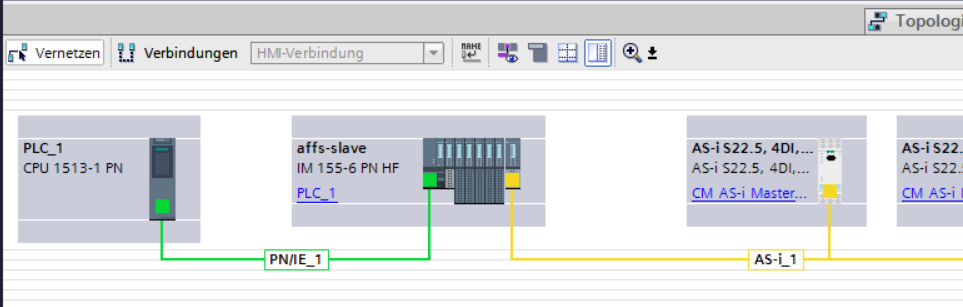
\includegraphics[width=0.9\textwidth]{Sensors/ASi_Geräteübersicht.png}
    \caption{Netzsicht im TIA-Portal mit ASi-Master und Slaves}
    \label{ASi-Netzansicht}
\end{figure}

Es ist besonders wichtig, dass in den Geräteeigenschaften der ET200SP die richtige Firmware-Version eingestellt ist, da sonst keine Verbindung zur Komponente hergestellt werden kann. Die Version der Firmware lässt sich in der Registerkarte Online-Zugänge unter \enquote{Online \& Diagnose} nachschauen, falls diese für das Gerät nicht bekannt ist. Unter \enquote{Slave Konfigurationstabelle} in den Geräteeigenschaften des ASi-Masters finden sich die den Slaves zugeteilten Eingangsadressen und ASi-Adressen. Die Adressen lassen sich hier auch ändern, was in erster Linie bei den ASi-Adressen benötigt wird, da diese nicht automatisch richtig eingestellt und nicht immer der Reihe nach zugeteilt werden. Die einem Slave zugeteilte Adresse kann an den Status-LEDs des ASi-Masters erlesen werden. An den LEDs \enquote{\mbox{SL\_Xy (A)}} und \enquote{\mbox{SL\_xY (B)}} lässt sich durch eine Blinkfolge die richtige Adresse herausfinden.\cite{ASi-Master_Handbuch}\\
Durch Verwendung einer Beobachtungstabelle lassen sich dann die Verbindungen zu den an den ASi-Slaves angeschlossenen Sensoren einfach überprüfen. Nach Einfügen der zugehörigen Eingangsadresse, Herstellen einer Online-Verbindung und Starten des Beobachtens wird das aktuelle Sensorsignal angezeigt.

\subsubsection{Verkabelung}
Insgesamt müssen 23 Sensoren über As-Interface mit der SPS verbunden werden. Die verwendeten ASi-Slaves haben jeweils vier Digitaleingänge (DI), wie auf Abb. \ref{ASi-Slaves} erkennbar ist, weshalb sechs Slaves benötigt werden würden. Da so jedoch manche Sensoren relativ weit von ihrem zugehörigen Slave entfernt wären, wird ein siebenter ASi-Slave verwendet, um Verkabelungsstrecken kurz halten zu können. Gewöhnlich wird zur ASi-Verbindung das in Kapitel \ref{par:ASi} beschriebene gelbe Profilkabel verwendet. Da die verwendeten Slaves aber nicht über den für das Kabel benötigten Anschluss verfügen, sondern nur eine jeweilige ASi-Plus und ASi-Minus Klemme besitzen, müssen diese über ein einfaches Kabel an den ASi-Master angeschlossen werden.\\
An den Slaves befindet sich jeweils nur ein ASi-Plus und -Minus Anschluss, weil die Slaves aber alle an die gemeinsamen Plus- und Minus-Leitungen angeschlossen werden müssen, und sich nicht mehrere Kabel in einen Anschluss befinden dürfen, musste eine Alternative zur Leitungsverbindung gefunden werden. Ursprünglich wurde eine zusätzliche Platine mit zwei dreipoligen Anschlussklemmen in Betracht gezogen. Da jedoch für die Befestigung der ASi-Slaves sowieso kleine Hutschienen am Lager angebracht werden mussten, und an diesen noch etwas Platz zur Verfügung stand, wurden auf diesen jeweils zwei Vier-Leiter-Reihenklemmen untergebracht. Über die Klemmen könnte daraufhin der jeweilige Slave mit der Plus- und Minus-Leitung verbunden werden.

\begin{figure}[H]
    \centering
    \begin{subfigure}{.4\textwidth}
        \centering
        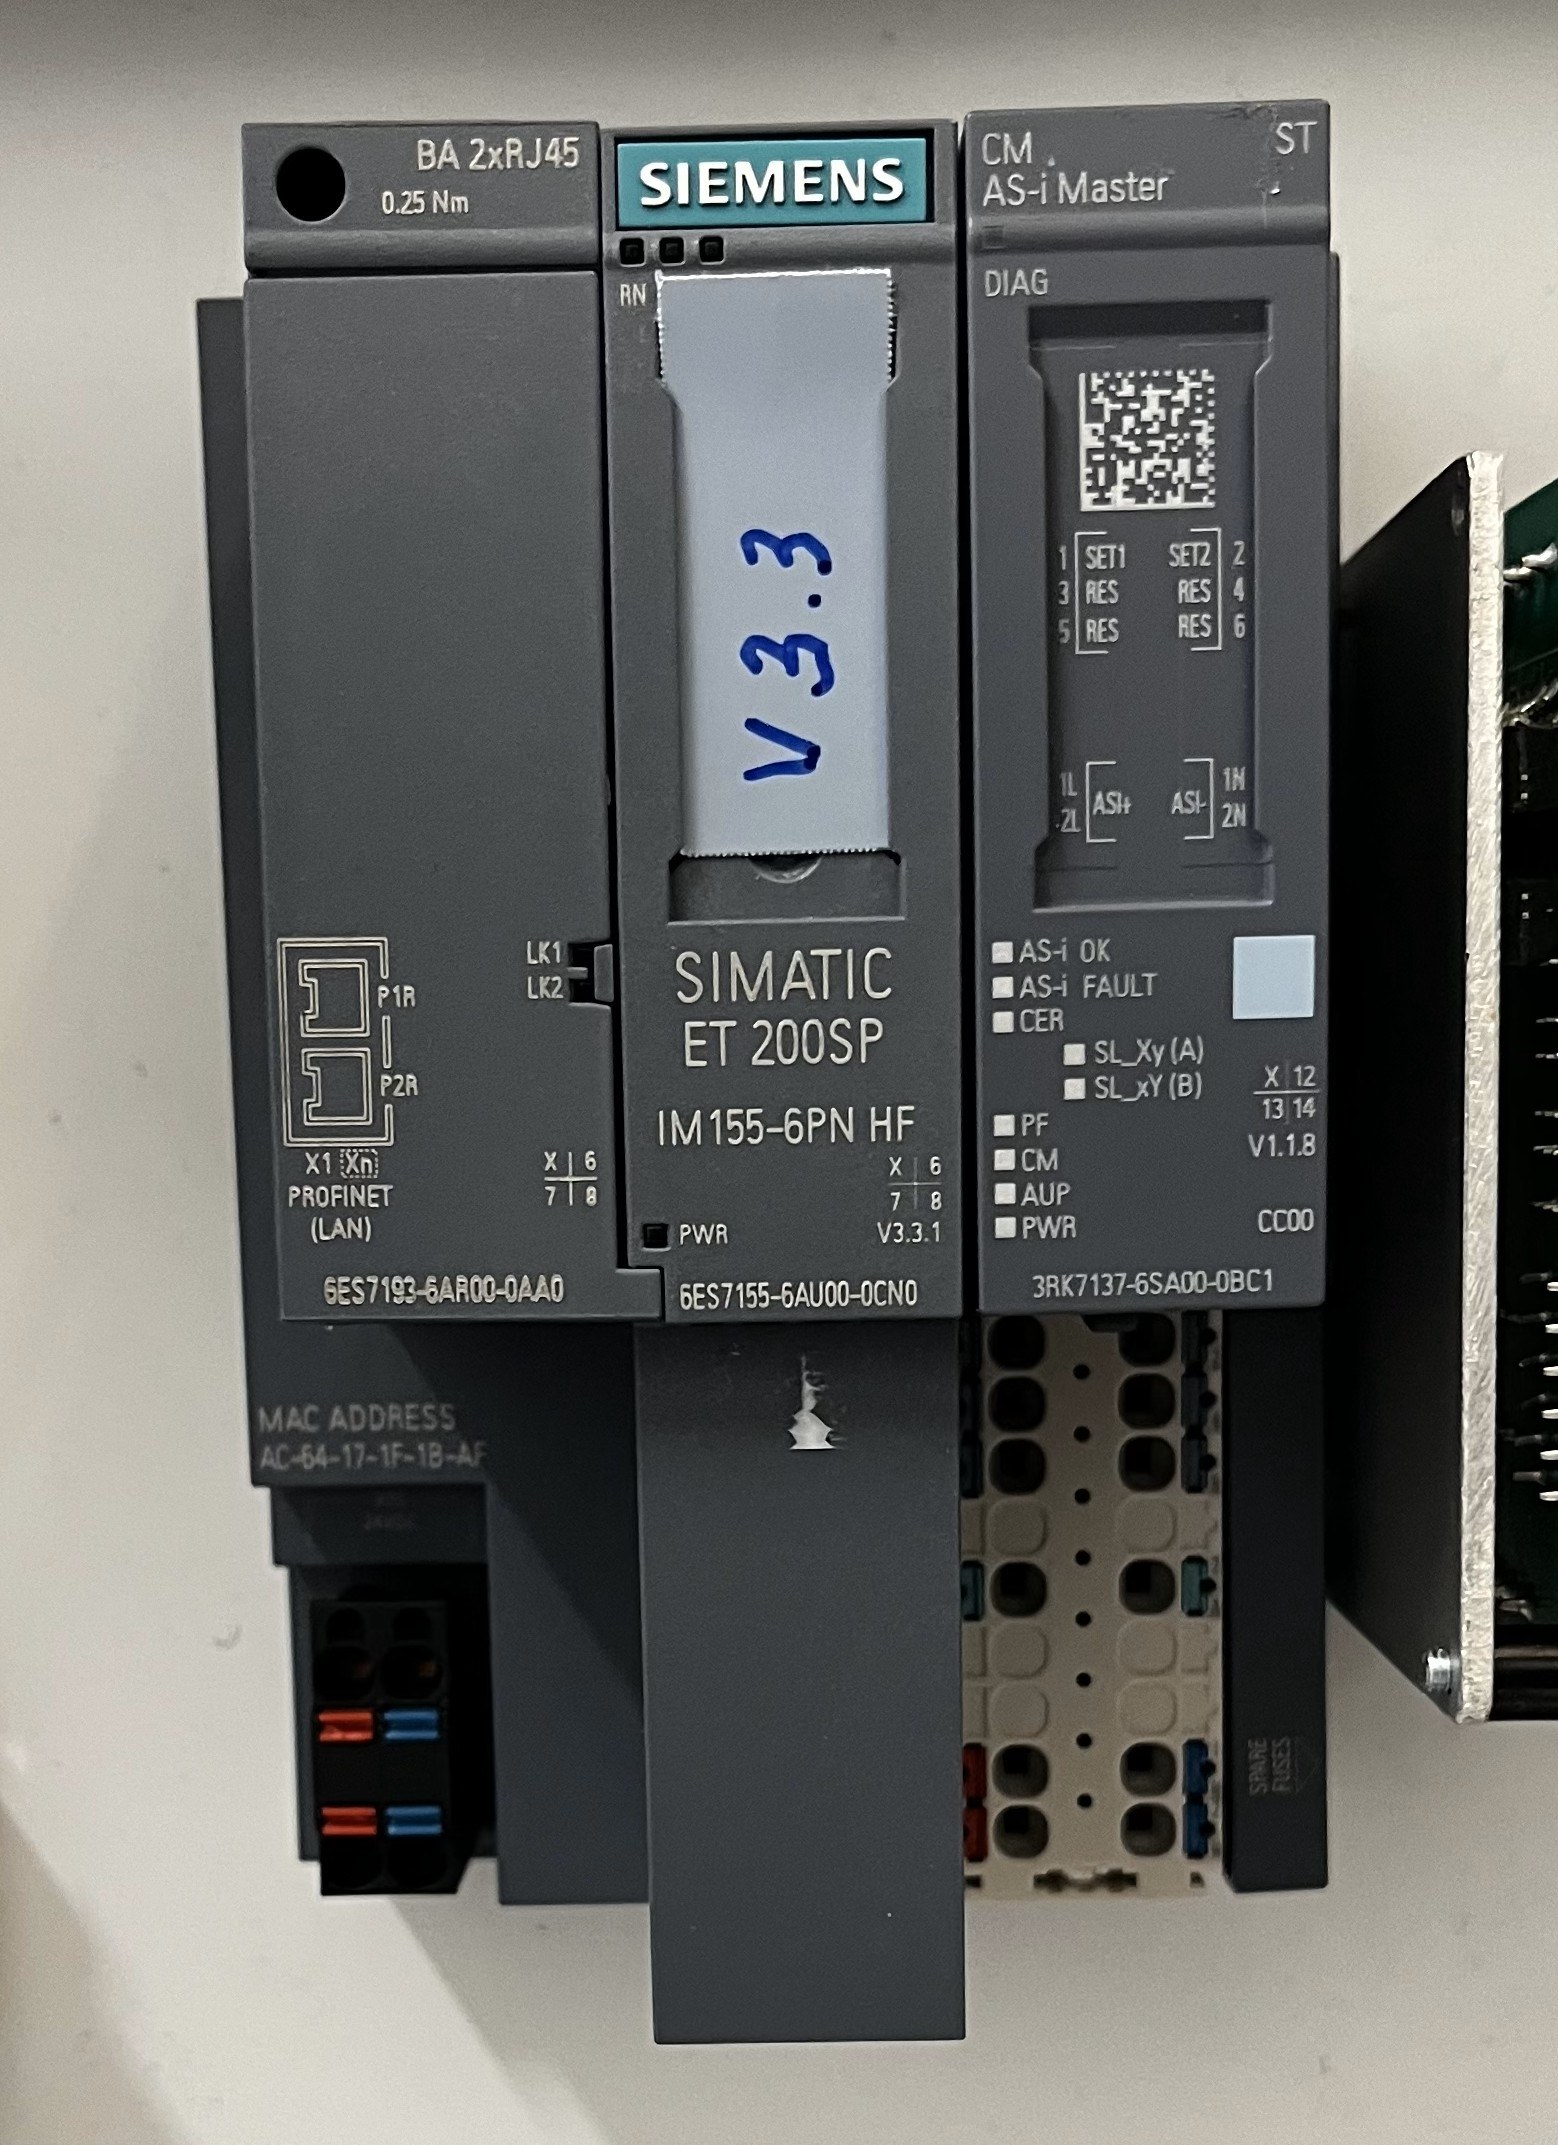
\includegraphics[width=0.71\textwidth]{Sensors/ET200SP.jpg}
        \caption{ET200SP mit ASi-Master Modul}
        \label{ET200SP}
    \end{subfigure}
    \begin{subfigure}{.4\textwidth}
        \centering
        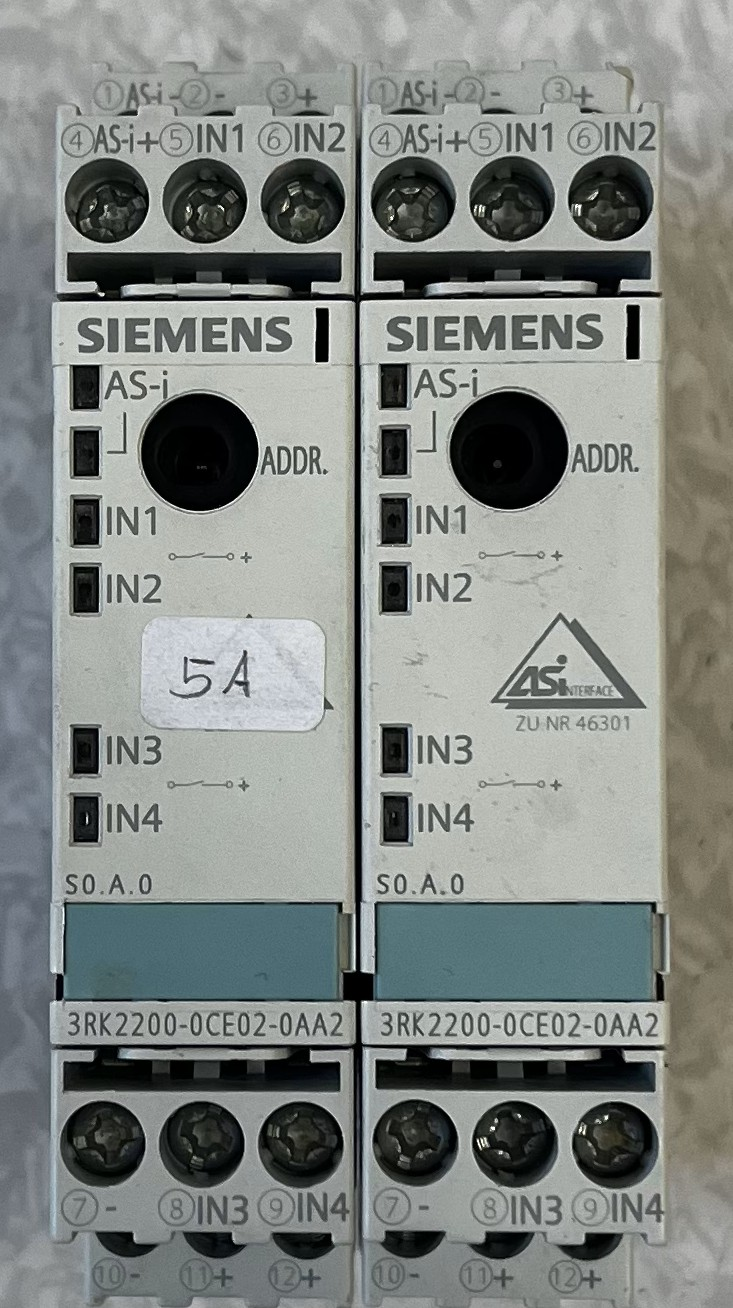
\includegraphics[width=0.58\textwidth]{Sensors/ASi-Slaves.jpg}
        \caption{ASi-Slaves}
        \label{ASi-Slaves}
    \end{subfigure}
    \caption{Siemens AS-Interface Komponente}
\end{figure}

Die Verbindung der Sensoren mit den jeweiligen Slaves besteht aus einer Plus-, Minus- und DI-Leitung. Ausgenommen sind die Endschalter mit Rollhebel, da diese nur einen Plus- und DI-Anschluss benötigen. Damit die Kabel für die Sensoren an den x-Achsen eng am Lager anliegen, wurden auf den Item-Profilen Kabelkanäle angebracht werden. Um die an den x-Achsen angebrachten querverbindenden Profile übergehen zu können, wurden eigene Kabelbrücken in Fusion360 gezeichnet und daraufhin 3D-gedruckt. Diese führen dann, wie in Abb. \ref{Kabelbrücke} ersichtlich, das Kabel oberhalb des Item-Profils entlang, ohne dass ein Knick entsteht.\\
An den ASi-Slaves befinden sich nur drei Plus- und drei Minus-Anschlüsse für die Sensoren. Da jedoch bei zwei von den sieben Slaves alle vier DI-Anschlüsse verwendet werden und alle angeschlossenen Sensoren eine Versorgung benötigen, müssen auch hier wieder Klemmen verwendet werden, um auch den vierten Sensor mit der Plus- und Minus-Leitung zu verbinden.

\begin{figure}[H]
    \centering
    \includegraphics[width=0.65\textwidth]{Sensors/Kabelbrücke.jpg}
    \caption{Kabelbrücke x-Achse}
    \label{Kabelbrücke}
\end{figure}

\subsection{Sicherheitstechnik}
\subsubsection{Aufgabenstellung}
Die Sicherheitstechnik soll so ausgelegt sein, dass beim Normalbetrieb keine Verletzungsgefahr für die Benutzerinnen und Benutzer besteht. Außerdem soll sie dafür sorgen, dass das System während des Betriebs sich selbst keinen Schaden zufügen kann. Zusätzlich soll sie Fehler, die durch menschliche Bedienung beim Einlagern entstehen können, minimieren. Somit kann die korrekte Funktion des AFSS über mehrere Jahre hinweg sicher gestellt werden.

\subsubsection{Personenschutz}\label{sc: Personenschutz}
Der Personenschutz hat die oberste Priorität. Er sorgt dafür, dass bei ordinärem Gebrauch die Benutzerinnen und Benutzer vor Verletzungen geschützt sind. Weiters soll er verhindern, dass Personen in elektrische Stromkreise geraten, oder mit unter Spannung stehenden Betriebsmitteln in Berührung kommen. Bei Wechselstrom mit \qty{50}{\hertz} liegt der in den Vorschriften festgelegte Grenzwert der Spannung, ab dem ein lebensgefährlicher Körperstrom fließen kann, bereits bei \qty{50}{\volt}. Bei Gleichstrom ist dieser Grenzwert bei \qty{120}{\volt} festgelegt.\cite{SeyrRösch} Durch den großen Strom wird die Signalleitung der Nerven und Muskeln gestört, und es kann zu Herzkammerflimmern sowie Atemproblemen kommen.\cite{Gefahr_el_Strom}\\
Für den Fall, dass eine Person trotz getroffener Sicherheitsvorkehrungen in den Stromkreis gerät, werden mehrere leicht zugängliche Not-Stop-Schalter am System angebracht, um schnell den Strom abschalten zu können. Als außenstehende Person ist es besonders wichtig, beim Entfernen der bereits in den Stromkreis geratenen Person, sich nicht selbst in Gefahr zu bringen oder auch in den Stromkreis zu kommen.\\
Als Abgrenzung zwischen Benutzerinnen und Benutzer und dem Schaltschrank ist dieser von außen versiegelt und lässt sich nur mit einem zugehörigen Schlüssel öffnen. Somit wird ein allseitiger Berührungsschutz sichergestellt und zusätzlich wird verhindert, dass Personen ohne Befugnis im Schaltschrank Änderungen durchführen können, und sich dabei womöglich verletzen. Im Schaltschrank befindet sich ein Fehlerstrom-Schutzschalter (FI), welcher bei \qty{30}{\milli\ampere} auslöst, und somit zum Personenschutz beiträgt.

\subsubsection{Schutz des Systems}
Damit auch umgekehrt das AFSS vor Fehlern durch Nutzerinnen und Nutzer geschützt ist, müssen auch hierfür eigene Sicherheitsvorkehrungen getroffen werden. Nur so kann für eine langjährige fehlerfreie Funktion des Systems gesorgt werden.
Da bereits für den Aufbau ein Raum genutzt wurde, der am Ende des Schuljahres wieder aufgeräumter verlassen werden muss und es durchaus möglich ist, dass das Lager und der Schaltschrank ihren Standort auch in Zukunft wieder wechseln müssen, wurden beide mit Rollen versehen. Durch anbringen der Rollen lässt sich das System problemlos durch das Schulgebäude transportieren ohne, dass es beim Raumwechsel zu einem Schaden kommt. Bereits bei der Planung des Lagers wurde miteinbezogen, dass das Lager die Höhe und Tiefe des Lifts im Werkstättengebäude nicht überschreiten darf, um den Transport in verschiedene Stockwerke zu ermöglichen. Auch die Höhen und Breiten der Türen im Gebäude wurden schon bei der Konstruktion berücksichtigt.\\
Das fertige Lagersystem soll planmäßig in der Factory der HTL untergebracht werden. Bei der Raumplanung stellte sich die Frage, ob das Bauteillager oder das Förderband an der Wandseite positioniert werden soll. Die Entscheidung fiel auf ersteres, um das System noch weiter Absichern zu können. Für den dazugehörigen Raumplan der Factory siehe Abb. \ref{}. Durch die Positionierung des Bauteillagers an der Wand wird es Schülerinnen und Schüler erschwert, selbst Bauteile auslagern zu können. Beim eigenhändigen Auslagern könnten leicht Boxen vertauscht werden, wodurch es bei Bestellung zu falschen Auslieferungen und Verwechslung von Bauteile kommen kann. Der manuelle Zugriff zum Lager wird durch das Förderband, welches wie eine Absperrung davor steht, verkompliziert.
\textbf{RAUMPLAN!!}
Für den Fall, dass ein händischer Zugriff zu den Bauteilen benötigt wird z.B. bei einem Stromausfall, lässt sich das Lager durch die darauf befestigten Rollen, mit etwas Aufwand, für den benötigten Zeitraum, an einen leichter zugänglichen Ort verschieben.\\
Das AFSS kann jedoch nicht nur durch den Menschen beschädigt werden, sonder auch sich selbst Schaden zufügen. Ziel der Sicherheitstechnik ist es auch in diesem Fall den verursachten Schaden zu minimieren und wenn möglich, sogar ganz zu verhindern. Einen weiteren wichtigen Teil zur Sicherheitstechnik trägt die am Lagersystem befestigte Sensorik bei. Damit die x-Schlitten oder das yz-Shuttle nicht in das Gerüst fahren können, und dieses dadurch beschädigen, befinden sich Endschalter auf jeder Achse. Wenn diese ausgelöst werden, wird das Technologieobjekt gesperrt und die Motoren werden sofort gestoppt. Außerdem wird durch das Referenzieren der Motoren bei jedem Neustart des Systems verhindert, dass sich die Koordinaten der Boxen verändern. Ansonsten könnte es passieren, dass Boxen, beim Versuch diese auszulagern, nicht richtig von der Gabel angehoben werden und auf den Boden fallen. Zusätzlich überprüfen die Lichttaster, ob die jeweilige Box während des Ein- und Auslagerungsprozesses an den Zwischenpositionen angekommen ist.\\
Nicht nur das Lager selbst, sondern auch die Antriebe und die sich im Schaltschrank befindenden Betriebsmittel müssen abgesichert werden. Falls ein zu hoher Strom fließt, zum Beispiel bei einem Kurzschluss, wird der Stromkreis durch einen Leitungsschutzschalter unterbrochen. Speziell für den Asynchronmotor des Fließbands wurde ein eigener Motorschütz eingebaut, um diesen vor Überstrom abzusichern. Weiters befinden sich drei Relais im Schaltschrank, die an die Enable-Kontakte der Motortreiberkarten angeschlossen wurden.\\
Es ist besonders wichtig, das AFSS auch für den Fall eines Stromausfalls abzusichern. Gefährdet wäre dadurch in erster Linie das yz-Shuttle. Wenn sich dieses irgendwo zwischen oberer und unterer x-Achse befindet, besteht bei einem Stromausfall die Gefahr, dass es durch die Schwerkraft einfach nach unten fällt. Durch die dabei entstehenden Kräfte könnte nicht nur das Shuttle selbst, sondern das ganze Gerüst des Lagers, beschädigt werden. Außerdem wird durch das drehen der Motoren in dessen Spulen ein Strom induziert, welcher in weiterer Folge Schäden an anderen Betriebsmitteln anrichten könnte. Da die verwendeten Schrittmotoren nicht mit eigenen Bremsen ausgestattet sind, musste ein eigenes Sicherheitskonzept entwickelt werden. Vor den Synchronmotoren der y-Achse werden Relais mit Wechslerkontakten eingebaut. Durch das Kurzschließen der Spulen des Motors wird verhindert, dass das Shuttle Richtung Boden fällt. Es wird dadurch abgebremst und bewegt sich langsam nach unten. Für eine ausführlichere Erklärung siehe Kapitel \ref{sec:Elektrische Planung}.

\subsection{Fazit}
Das AFSS umfasst insgesamt sechs verschiedene Arten von Sensoren, die alle ihren jeweiligen Anforderungen entsprechend ausgewählt und mit dem SPS-Programm verbunden wurden. Zum Referenzieren musste für den verwendeten Sensor eine passende Schaltung und Platine entworfen werden, dessen Herstellung durch die schulinterne Leiterplattenfertigung ermöglicht wurde. Zur Kommunikation zwischen Sensoren und SPS wurde AS-Interface verwendet, ausgenommen des Barcodescanners. ASi konnte erfolgreich in das TIA-Portal eingebunden werden, damit die Signalverarbeitung der Sensoren und die Steuerung der Motoren in einem gemeinsamen Programm stattfinden kann.\\
Durch die integrierten Sicherheitskonzepte können Schäden am System stark vermieden werden. Auch für den Fall, dass es zu einer gefährlichen Situation kommen sollte, wurden Sicherheitsvorkehrungen getroffen, um die entstehenden Schäden durch sofortiges Stoppen des Systems minimieren zu können. Vor allem die Absicherung des yz-Shuttles bei einem Stromausfall musste gut durchdacht werden, aber auch hierfür konnte eine sichere Lösung gefunden werden. Die wichtigste Anforderung war der Personenschutz, welcher sichergestellt werden konnte.